\documentclass[12pt,letterpaper]{article}

\usepackage{amsmath, amsthm, amsfonts, amssymb}
\usepackage{microtype, parskip, graphicx}
\usepackage[comma,numbers,sort&compress]{natbib}
\usepackage{lineno}
\usepackage{longtable}
\usepackage{docmute}
\usepackage{caption, subcaption, multirow, morefloats, rotating}
\usepackage{wrapfig}
\usepackage{hyperref}

\frenchspacing

\begin{document}

\section{Data Specifications}

We analyzed microfossil occurrence information which was downloaded from the Neptune Database \url{http://www.nsb-mfn-berlin.de/nannotax}. We downloaded all occurrence information for calcareous nannofossils, diatoms, foraminifera, and radiolarians from the entire globe and having occurred between 120 and 0 Mya. This selection of occurrences was then culled to just those species which have their first occurrence at most 63 My; this avoids those taxa which survived the K/Pg boundary, those taxa arising just after the K/Pg boundary, and lines up the occurrences with the temperature time-series (discussed below).

All occurrences were binned into 1 My bins based on the estimated age of the fossil occurrence. Because the estimated ages of each occurrence is a product of core-specific age-models and can be overly precise, the hope is that by binning the data this smooths over the between-core heterogeneity and thus homogenizes our disparate data sources. We then determined for each species the million year bins when it had occurred. For every occurrence of a species, except the last, that species is considered to have survived and was marked with a 0. The last occurrence of that species is considered the bin in which the taxon has gone extinct. This protocol means that we are reading the fossil record ``as written,'' a practice that is potentially dangerous as it is a overconfident statement of preservation and may be shortening the actual duration of that species CITATIONS. However, this practice is common with marine microfossil data CITATIONS.

A taxon's geographic range was calculated for each of the 1 My bins in which it occurred. Geographic range was calculated as the maximum great circle distance on an ellipsoid (i.e. the globe) between any two occurrences; this measure is also called a geodesic. This distance was measured in kilometers. The geodesic distance was then log-plus-one transformed and then standardized by zero-centering the data and then dividing by its standard deviation so that geographic range had mean 0 and standard deviation 1. This standardization means that a regression coefficient associated with this covariate describes the change in extinction probability per change in standard deviation of geographic range, and that coefficients associated with similarly standardized covariates will be directly comparable in magnitude.

Temperature data used as covariates in this analysis are based on Magnesium/Calcium isotope ratios sourced from Cramer et al CITATION. These are considered a more accurate estimate of global temperature than the standard Oxygen isotope-based estimates because Mg/Ca based estimates are not effected by ice-volume and fresh-water input (e.g. meteoric water). This property is of particular importance for this analysis as polar ice-caps develop midway through the Cenozoic. Our data source, Cramer et al., provides temperature estimates for every 0.1 My from 0 to 63 Mya. We binned these estimates into 1 My intervals as we did with the fossil occurrences. The temperature estimate for each 1 My interval was calculated as the mean of all estimates within that interval (Fig. \ref{fig:temp_curve}). Temperature was then transformed and standardized the in the same manner as geographic range (above).

\begin{figure}[ht]
  \centering
  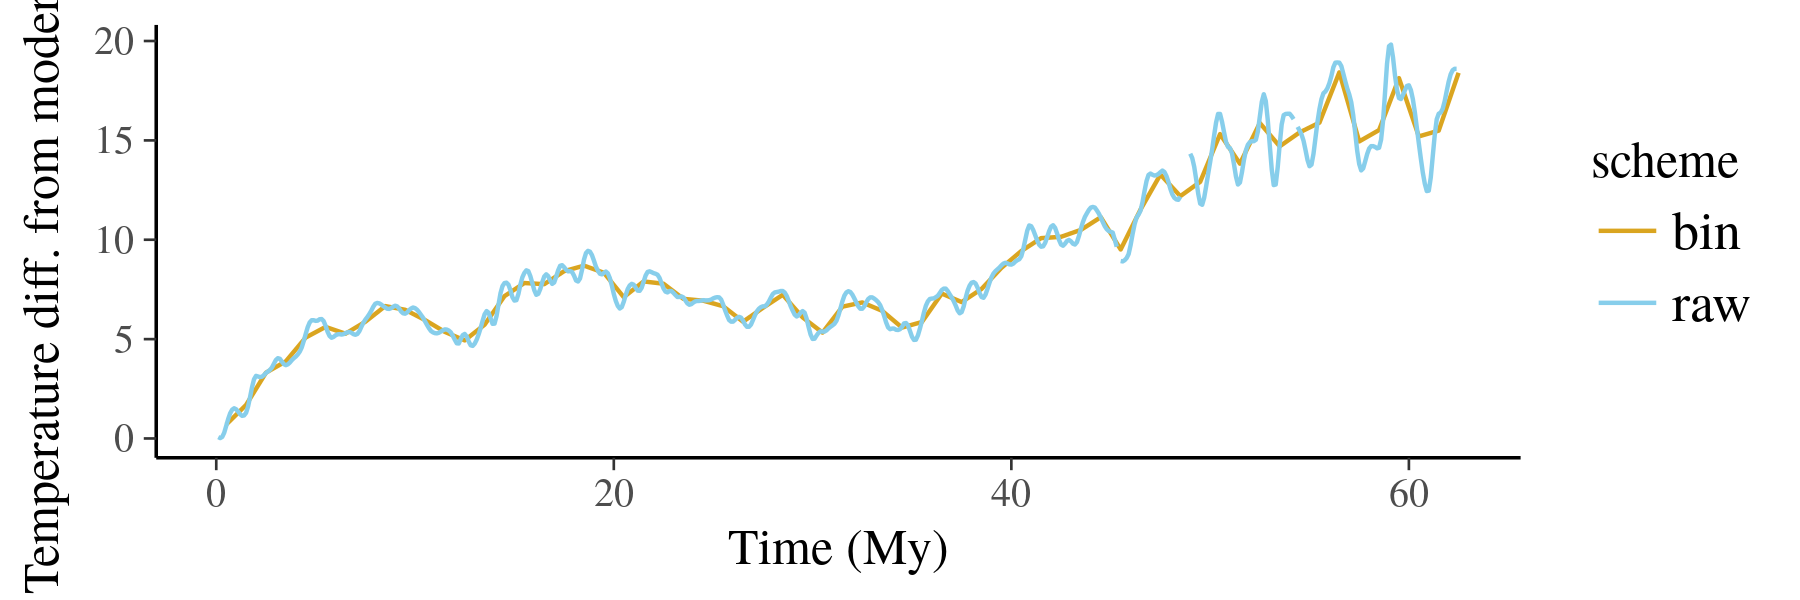
\includegraphics[width=\textwidth,height=0.5\textheight,keepaspectratio=true]{figure/cramer_temp}
  \caption{Comparison of initial temperature estimates from Cramer et al. CITATION (goldenrod) versus the binned values used in this analysis (blue). The initial values are for every 0.1 My while our bins are defined for every 1 My.}
  \label{fig:temp_curve}
\end{figure}


\section{Model Specifications}

In survival analysis, the hazard function describes the instantaneous rate of extinction of a species given its age and relevant covariates. The hazard function is defined as the conditional probability of a species going extinct by the end of the \(t\)-th interval given that it survived up until \(t\) and the relevant covariate information \(X\) for all \(k\) 1 My intervals. For the discrete time intervals \(T = 1, \cdots, k\), extinction is defined as \(T = t\). The discrete time hazard function is defined as
\begin{equation}
  \lambda(t | X) = P(T = t | T \geq t, X), \quad t = 1, \cdots, k. \\
  \label{eq:hazard}
\end{equation}

%The complement of the hazard function is called the survival function, which describes the probability of a species going extinct after time \(t\). Just as extinction is defined as when the current occurrence is the last occurrence, or \(T = t\), survival is defined as when the current occurrence is less than (in age) than the final occurrence, or \(T > t\). The discrete time survival function is expressed as
%\begin{equation}
%  S(t | X) = P(T > t | X) = \prod{i = 1}{t}(1 - \lambda(i | X).
%  \label{eq:surv}
%\end{equation}

The hazard function (Eq. \ref{eq:hazard}) is easily reparameterized as a logistic regression by defining that \(\lambda(t | X) = h(\Theta)\) where \(h(.)\) is a logit inverse-link function and \(\Theta\) is the probability of a taxon going extinction during interval \(t\). \(h(\Theta)\) is then modeled as with any regression as it is defined for all real-values. In this case, we opted for a hierarchical/mixed-effects model with multiple non-nested varying intercepts and slopes CITATION. 

Our covariates matrix \(X\) is a \(N \times D\) matrix where \(N\) is the total number of observations and \(D\) is the total number of covariates. The first column of \(X\) is entirely 1's as it corresponds to the intercept term in the regression model. The next two columns of \(X\) are two aspects of geographic range as continuous covariates: geographic range \(r\) during interval \(t\), and the difference \(d\) between the geographic range at \(t - 1\) and \(t\). The difference in geographic range was calculated from the transformed and standardized geographic range values; this means that change in geographic range is in units of changes in standard deviations. The final two columns are two aspects of global temperature: mean temperature during interval \(t\), and the lag of mean temperature (i.e. mean temperature during interval \(t - 1\).) As with change to geographic range, the lag of temperature is based on the transformed and standardized temperature estimates. 

The matrix of time and phylum varying regression coefficients describing the effects of the covariates on a species' risk of extinction is called \(B\). These regression coefficients are themselves modeled as being multivariate normally distributed with vector of means \(\alpha\) describing the average intercept and regression coefficient estimates of each coefficients for each phylum \(p\). These phylum averages are themselves modeled as multivariate normally distributed with mean vector \(\mu\) describing the overall average regression coefficients, including the intercept. 

This logistic regression model, minus the final selection of priors, is expressed as 
\begin{equation}
  \begin{aligned}
    t_{i} &\sim \text{Bernoulli}(\Theta) \\
    \Theta_{i} &= \text{logit}^{-1} (X_{i} B_{w[i], p[i]} + a_{d[i], p[i]}) \\
    B_{w, p} &\sim MVN(\alpha_{p}, \Sigma_{B}) \\
    \alpha_{p} &\sim MVN(\mu, \Sigma_{\alpha}) \\
    a_{w, p} &\sim MVN(\delta_{p}, \Sigma_{a}) \\
    \delta_{p} &\sim MVN(0, \Sigma_{\delta}) \\
  \end{aligned}
  \label{eq:core}
\end{equation}
with \(i\) indexing the observation and bracket subscripts referencing the class of the \(i\)th observation where \(w[i]\) is the time of the \(i\)-th observation, \(p[i]\) is the phylum of the \(i\)-th observation, and \(d[i]\) is the age of the \(i\)-th observation. 

To complete the generative model, we need to assign final priors to the ``top level'' parameters
\begin{equation}
  \begin{aligned}
    \mu_{c} &\sim 
      \begin{cases}
        N(0, 10) & \text{if } c = 1 \\
        N(0, 3) & \text{if } c > 1 \\
      \end{cases}
    \delta &\sim N(0, 1) \\
    \Sigma_{B} &= diag(\tau_{B}) \Omega_{B} diag(\tau_{B}) \\
    \Sigma_{\alpha} &= diag(\tau_{\alpha}) \Omega_{\alpha} diag(\tau_{\alpha}) \\
    \Sigma_{a} &= diag(\tau_{a}) \Omega_{a} diag(\tau_{a}) \\
    \Sigma_{\delta} &= diag(\tau_{\delta}) \Omega_{\delta} diag(\tau_{\delta}) \\
    \tau_{B} &\sim C^{+}(5) \\
    \tau_{\alpha} &\sim C^{+}(5) \\
    \tau_{a} &\sim C^{+}(5) \\
    \tau_{\delta} &\sim C^{+}(5) \\
    \Omega_{B} &\sim LKJ(1) \\
    \Omega_{\alpha} &\sim LKJ(1) \\
    \Omega_{a} &\sim LKJ(1) \\
    \Omega_{\delta} &\sim LKJ(1). \\
  \end{aligned}
  \label{eq:priors}
\end{equation}
The decomposition of the covariance matrices (e.g \(\Sigma_{B}\)) allows priors the variance and correlation aspects of covariance to be defined separately. These priors are also slightly more interpretable than a, for example, inverse-Wishart distributed prior for the covariance matrices. This decomposition is recommended by CITATION.


\section{Model Parameter Estimation}

We implemented our model using the \begin{texttt}rstanarm\end{texttt} package for the R programming language CITATION. This package provides an interface to the Stan probabilistic programming language for writing hierarchical/mixed-effects models in native R. Posterior estimates were obtained through Hamiltonian Monte Carlo, using 2000 steps divided equally between warm-up and sampling. In order to prevent divergent transitions the adapt delta value was increased to 0.99; all other HMC/NUTS sampling parameters were kept at the defaults for rstanarm version XX CITATION. An example line of R code to fit this mode given a data.frame of all necessary data called ``data'' could be written as:
\begin{verbatim}
  stan_glmer(formula = event ~ range + range_diff + temp + temp_lag + 
                       (1 + range + range_diff | mybin/phylum) + 
                       (1 | age/phylum), 
             prior = normal(0, 3, autoscale = FALSE), 
             prior_intercept = normal(0, 10, autoscale = FALSE), 
             prior_aux = cauchy(0, 5, autoscale = FALSE), 
             data = data, 
             adapt_delta = 0.99, 
             thin = 4)
\end{verbatim}

Posterior convergence was determined using the following general and HMC specific diagnostic criteria: scale reduction factor (\(\hat{R}\); target \(<1.1\)), effective sample size (eff; target value eff/steps \(<0.0001\)), number of samples that saturated the maximum trajectory length for avoiding infinite loops (treedepth; target value 0), sample divergence, and the energy Bayesian Fraction of Mission Information (E-BFMI; target value \(>0.2\)). For further explanation of these diagnostic criteria, see the Stan Manual CITATION.


\section{Model Selection and Adequacy}

We considered four variants of this model: 1) historical covariates with time-varying intercepts and slopes, 2) no historical coviarates with time-varying intercepts and slopes, 3) historical covariates without time-varying intercepts and slopes, and 4) no historical covariates and no time-varying intercepts and slopes (except age effect).

To determine how many non-nested varying-intercept terms were possible to include without overly biasing out models' parameter estimates, the four variant models described above were compared using both WAIC and LOOIC which are estimates of a model's expected out-of-sample performance; these measures are fully Bayesian, taking into account the entire estimated joint posterior CITATION. WAIC and LOOIC are interpreted similarly to AIC, with lower values indicating greater expected out-of-sample performance. Additionally, the Bayesian nature of WAIC and LOOIC mean that they are calculated with standard errors allowing for a more nuanced understanding the actual amount of difference between the models. We selected the model with the lowest WAIC and LOOIC, which happened to be are most parameter rich model.

Model adequacy was measured using the area under the receiver operating characteristic curve (AUC). This measure is commonly used in classification problems like this one as it has the desirable characteristic of comparing the model's true positive rate with its false positive rate, as opposed to only true positive rate measured by accuracy CITATION. This value ranges between 0.5 and 1, with 0.5 indicating no improvement in performance from random and 1 indicating perfect performance. AUC was calculated for the dataset as a whole, and for each of time bins. These values are measures of in-sample predictive accuracy.


\subsection{Prediction given class imbalance}

One of the issues with our data set is extreme class imbalance; this means that there are many more survival observations than extinction observations. When the classes are not approximately balanced, the base probability of 1 versus 0 is below 0.5. When the intercept term of the logistic regression is sufficiently negative (-2 or less), the only way to obtain a linear predictor value of 0.5 or greater is if the covariate effects are large or there the covariates are at extreme values. The 0.5 default cut-off point for binary prediction is much to high when events are rare. A method for determining the new ``optimal'' cut-point involves calculating the receiver operating characterist (ROC) curve from the linear predictor estimates and then identifying the point on the ROC curve which maximizes both true positive rate and the false positive rate. The new cut-point is then back-calculated from the true positive and false positive rates. Class membership is then predicted given this new cut-point. This process is done for every posterior draw, as each realization from the posterior predictive distribution has its own optimal cut-point.

\subsection{Cross-validation}

In addition to model selection and adequacy, we are also interested in understanding how well our model predicts species extinction given new,future data. We estimated out-of-sample predictive error using cross-validation. For our dataset, expected out-of-sample AUC was estimated using five-fold cross-validation. For time-series data, the folds (data partitions) are approximately equal segments of time. The model is fit to the first fold and the posterior estimates are used to predict the states of the observations in the second fold, then the model is fit to the first and second fold and the posterior states are used to estimate the states from the third fold, and so on with increasingly large numbers of folds used for fitting a model to predict the states from the subsequent fold. With 63 time points, each of the five folds represents approximately 13 time points. Keep in mind, however, that each time point corresponds to many (100-1000) individual observations.

For each posterior draw of the cross-validation predictions, the optimal cut-point was calculated as described above. Given these class assignments based on estimated optimal cut-point, the AUC value of the out-of-sample estimates was calculated. AUC values are calculated for the entire fold and for each of the individual time points represented within that fold.

See our code repository LINK for full code details. Our code uses ``tidyverse'' tools such as dplyr CITATION, purr CITATION, and tidybayes CITATION, thus some familiarity with that package ecosystem is necessary to fully comprehend how we've processed our data and results.

\end{document}
